\section{Pure Virtual}
In dieser Aufgabe wollen wir Vererbung und Polymorphie dazu nutzen, um mathematische Ausdrücke als Bäume von Primitivoperationen zu modellieren.
Dazu werden wir eine abstrakte Oberklasse \lstinline{Expression} mit der abstrakten Methode \lstinline{compute()} erstellen.
Einzelne Knotentypen wie Addition und Subtraktion werden von \lstinline{Expression} abgeleitet und implementieren \lstinline{compute()}, um die jeweilige Operation zu realisieren.
\begin{figure}[h]
\begin{center}
	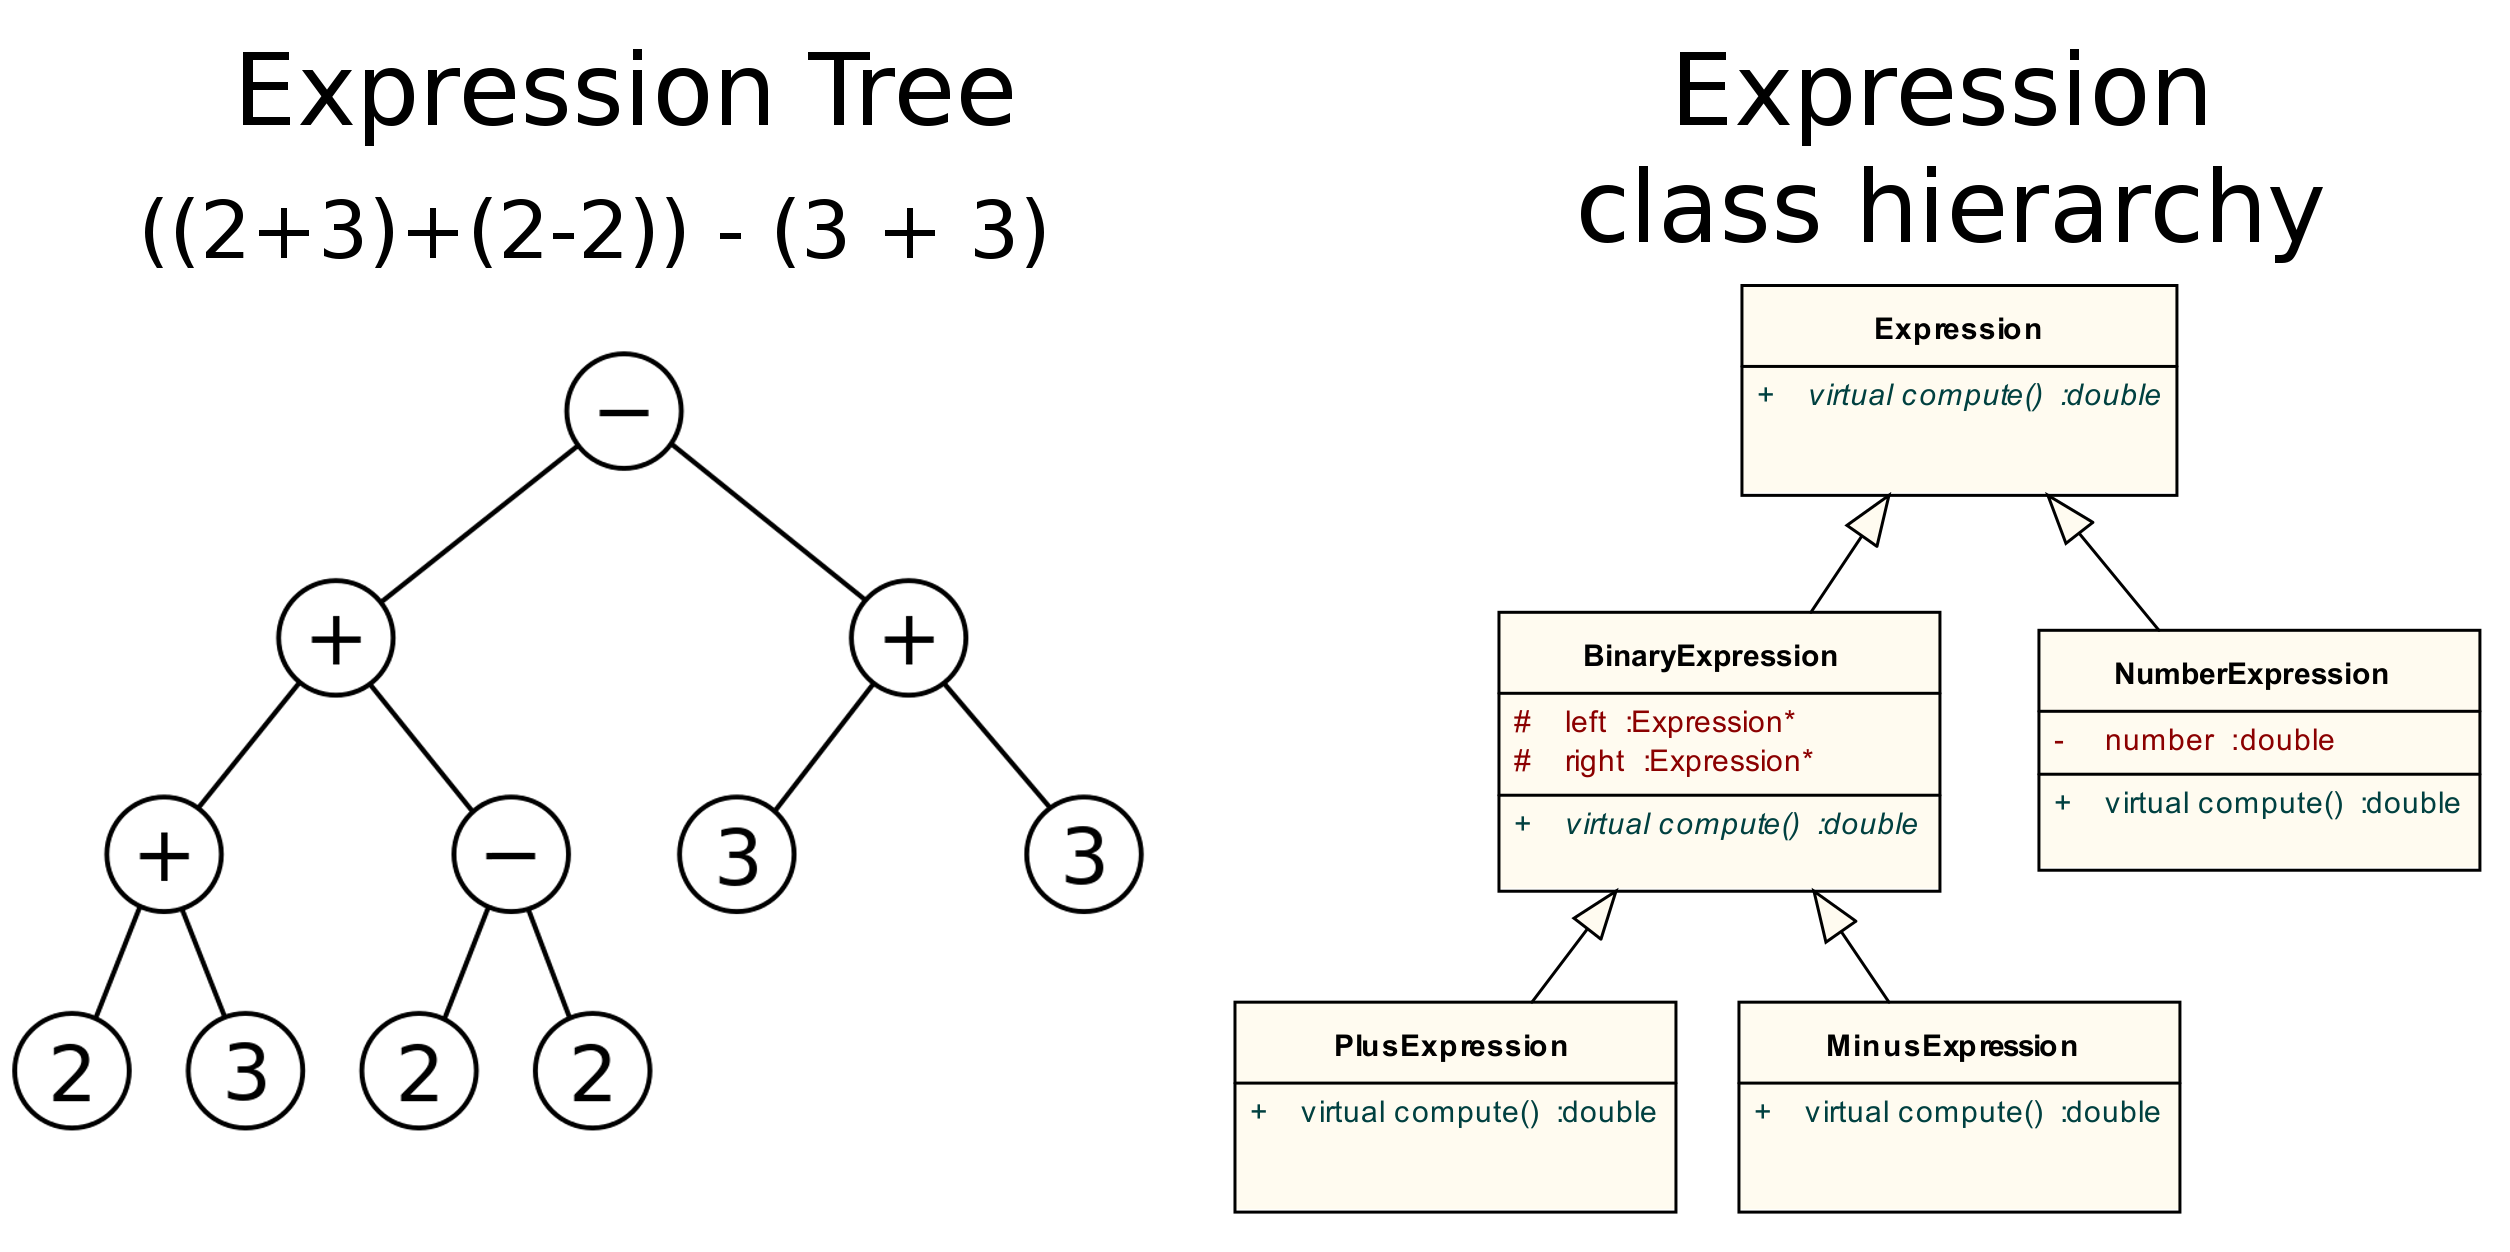
\includegraphics[width=.75\textwidth]{figures/ExpressionTree.png}\\
	\caption{Beispielausdruck mit Ausdrucksbaum und Klassenhierarchie}
\end{center}
\end{figure}


\begin{enumerate}

\item \textbf{Klasse \lstinline{Expression}:}
Schreibe die abstrakte Klasse \lstinline{Expression}.
Diese soll als Basisklasse für alle Ausdrücke dienen.
Implementiere einen parameterlosen Konstruktor und einen virtuellen Destruktor, die je eine Meldung auf der Konsole ausgeben, sodass es bei der Ausführung ersichtlich wird, wann eine \lstinline{Expression} erzeugt und wann zerstört wird.
Deklariere außerdem eine abstrakte (pure \lstinline{virtual}) Methode \lstinline{virtual double compute() = 0;}, die das Ergebnis des Ausdrucks berechnen und zurückgeben soll.
\hints{
    \item Anders als in Java muss die Klasse nicht explizit als \lstinline{abstract} gekennzeichnet werden - es reicht, wenn sie mindestens eine \emph{pure virtual} Methode enthält.
} 

\item \textbf{Klasse \lstinline{NumberExpression}:}
Schreibe die Klasse \lstinline{NumberExpression}, die ein (Baum-)Blatt mit einer Zahl darstellt.
Dementsprechend soll \lstinline{NumberExpression} von \lstinline{Expression} erben und ein Attribut zum Speichern einer Zahl besitzen, das im Konstruktor initialisiert wird.
Implementiere den Konstruktor und virtuellen Destruktor und versehe auch diese mit einer Konsolenausgabe.
Die Methode \lstinline{compute()} gibt die gespeicherte Zahl zurück.

\item \textbf{Klasse \lstinline{BinaryExpression}:}
Schreibe die abstrakte Klasse \lstinline{BinaryExpression} mit den \lstinline{protected} Attributen \lstinline{Expression *left, *right}.
Implementiere den Konstruktor und virtuellen Destruktor mit entsprechender Ausgabe.

\item \textbf{Klassen \lstinline{PlusExpression} und \lstinline{MinusExpression}:}
Schreibe die Klassen \lstinline{PlusExpression} und \lstinline{MinusExpression}, die von \lstinline{BinaryExpression} erben und eine Addition bzw. Subtraktion realisieren. 
Implementiere die Kon- und Destruktoren sowie die \lstinline{compute()} Methode.

\item \textbf{Testlauf:}
Teste deine Implementation.
Ein gutes Beispiel findest du in Abbildung weiter oben.
Schaue dir die Ausgabe genau an und versuche anhand der gegebenen Klassenhierarchie die Reihenfolge der Erzeugung und Zerstörung von Objekten  nachzuvollziehen.

\end{enumerate}
